\chapter{Mappatura}
\rhead[\fancyplain{}{\bfseries \thechapter \:Mappatura}]
{\fancyplain{}{\bfseries\thepage}}

In questa Appendice viene riportata la mappatura effettiva applicata per la conversione del dataset XML da \emph{Scheda F} a \emph{CIDOC-CRM}.\\
Per compattezza sono state omesse le proprietà basilari (e.g. \emph{rdfs:label}) desumibili dal codice.

Per confronto e completezza è stata inclusa anche l'iniziale mappatura teorica, in seguito modificata a fronte delle strutture reali.

\begin{center}
\tiny

\begin{longtable}{ | p{1cm} | p{8cm} | p{3cm} | }
\caption{Mappatura effettiva da Scheda F a CIDOC-CRM} \label{tab:schedaf-to-owl} \\
\hline \multicolumn{1}{|p{1cm}|}{\cellcolor{lightyellow}\textbf{Campo Scheda F}} & \multicolumn{1}{p{8cm}|}{\cellcolor{lightyellow}\textbf{mappatura CIDOC-CRM}} & \multicolumn{1}{p{3cm}|}{\cellcolor{lightyellow}\textbf{Note}}\\ \hline
\endfirsthead
\multicolumn{3}{c}%
{{\bfseries \tablename\ \thetable{} -- continua da pag. precedente}} \\
\hline \multicolumn{1}{|p{1cm}|}{\cellcolor{lightyellow}\textbf{Campo Scheda F}} & \multicolumn{1}{p{8cm}|}{\cellcolor{lightyellow}\textbf{mappatura CIDOC-CRM}} & \multicolumn{1}{p{3cm}|}{\cellcolor{lightyellow}\textbf{Note}} \\ \hline
\endhead
\hline \multicolumn{3}{r}{{continua a pag. successiva}}\\
\endfoot
\hline \hline
\endlastfoot

  \multicolumn{3}{|l|}{\cellcolor{lightcyan}COPYRIGHT}\\ \hline
  CRPD & entry - CRM.P104\_is\_subject\_to - CRM.E30\_Right & \\
  & CRM.P3 has note - Literal & \\ \hline

  \multicolumn{3}{|l|}{\cellcolor{lightcyan}NOTES}\\ \hline
  OSS &  entry - CRM.P3\_has\_note - Literal & \\ \hline

  \multicolumn{3}{|l|}{\cellcolor{lightcyan}SUPERVISOR}\\ \hline
  FUR &  entry - CRM.P94i\_was\_created\_by - CRM.E65\_Creation & \\
   & CRM.P11\_had\_participant - CRM.E39\_Actor & \\ \hline
  
  \multicolumn{3}{|l|}{\cellcolor{lightcyan}CLASSIFICATION}\\ \hline
  SERCDOA &  entry - CRM.P67\_refers\_to - CRM.E31\_Document & \\ \hline
  INVN &  photo - CRM.P149\_is\_identified\_by - CRM.E42\_Identifier & \\ \hline
  \pagebreak
  UBFP &  photo - CRM.P54\_has\_current\_permanent\_location - CRM.E53\_Place & \multirow{12}{3cm}{UBFP, UBFS, UBFT e UBFU sono collocazioni annidate, perciò il CRM.E53\_Place più interno è inscatolato nel più esterno tramite CRM.P59i} \\
   & CRM.P87\_is\_identified\_by - CRM.E44\_Place\_Appellation & \\
   & CRM.P59i\_is\_located\_on\_or\_within - CRM.E53\_Place & \\ \cline{1-2}
  UBFS &  photo - CRM.P54\_has\_current\_permanent\_location - CRM.E53\_Place & \\
   & CRM.P87\_is\_identified\_by - CRM.E44\_Place\_Appellation & \\
   & CRM.P59i\_is\_located\_on\_or\_within - CRM.E53\_Place & \\ \cline{1-2}
  UBFT &  photo - CRM.P54\_has\_current\_permanent\_location - CRM.E53\_Place & \\
   & CRM.P87\_is\_identified\_by - CRM.E44\_Place\_Appellation & \\
   & CRM.P59i\_is\_located\_on\_or\_within - CRM.E53\_Place & \\ \cline{1-2}
  UBFU &  photo - CRM.P54\_has\_current\_permanent\_location - CRM.E53\_Place & \\
   & CRM.P87\_is\_identified\_by - CRM.E44\_Place\_Appellation & \\
   & CRM.P59i\_is\_located\_on\_or\_within - CRM.E53\_Place & \\ \hline
  
  \multicolumn{3}{|l|}{\cellcolor{lightcyan}OWNERSHIP}\\ \hline
  CDGG &  photo - CRM.P24i\_changed\_ownership\_through - CRM.E8\_Acquisition & \\
   & CRM.P3\_has\_note - Literal & \\ \hline
  CDGS &  photo - CRM.P24i\_changed\_ownership\_through - CRM.E8\_Acquisition & \\
   & CRM.P22\_transferred\_title\_to - CRM.E39\_Actor & \\ \hline
  
  \multicolumn{3}{|l|}{\cellcolor{lightcyan}CODES}\\ \hline
  TSK &  entry - CRM.P2i\_is\_type\_of - CRM.E55\_Type & \\ \hline
  NCTN &  entry - CRM.P48\_has\_preferred\_identifier - CRM.E42\_Identifier & \\
   & CRM.P2\_has\_type - CRM.E55\_Type & type: id\_number \\ \hline
  NCTR &  entry - CRM.P48\_has\_preferred\_identifier - CRM.E42\_Identifier & \\
   & CRM.P2\_has\_type - CRM.E55\_Type & type: regional\_code \\ \hline
  ESC & entry - CRM.P50\_has\_current\_keeper - CRM.E40\_Legal\_Body & \\ \hline
  
  \multicolumn{3}{|l|}{\cellcolor{lightcyan}CATALOGUING}\\ \hline
  CMPD &  entry - CRM.P94i\_was\_created\_by - CRM.E65\_Creation & \\
   & CRM.P4\_has\_time-span - CRM.E52\_Time-Span & \\
   & CRM.P78\_is\_identified\_by - CRM.E49\_Time\_Appellation & \\ \hline
  CMPN &  entry - CRM.P94i\_was\_created\_by - CRM.E65\_Creation & \\
   & CRM.P14\_carried\_out\_by - CRM.E39\_Actor & \\ \hline
  
  \multicolumn{3}{|l|}{\cellcolor{lightcyan}UPDATING (ripetibile)}\\ \hline
  AGGD &  entry - CRM.P124i\_was\_transformed\_by - CRM.E81\_Transformation & \\
   & CRM.P4\_has\_time-span - CRM.E52\_Time-Span & \\
   & CRM.P78\_is\_identified\_by - CRM.E49\_Time\_Appellation & \\ \hline
  AGGN &  entry - CRM.P124i\_was\_transformed\_by - CRM.E81\_Transformation & \\
   & CRM.P11\_had\_participant - CRM.E39\_Actor & \\ \hline

  \multicolumn{3}{|l|}{\cellcolor{lightcyan}OBJECT}\\ \hline
  OGTD &  photo - CRM.P2\_has\_type - CRM.E55\_Type & \\ \hline
  QNTN &  photo - CRM.P57\_has\_number\_of\_parts - Literal & \\ \hline
  OGTB &  photo - DC.type - Literal & \\ \hline
  OGTS &  photo - DC.format - CRM.E55\_Type & formato oggetto fotog. \\ \hline
  MTX &  photo - DC.format - CRM.E55\_Type & bn/colore \\ \hline
  MTC &  photo - CRM.P45\_consists\_of - CRM.E55\_Type & \\ \hline
  \multirow{5}{1cm}{MISA\\MISL\\MISD\\(MISU)\\(MISO)} &  photo - CRM.P43\_has\_dimension - CRM.E54\_Dimension & \multirow{5}{3cm}{per ogni tipo di dimensione viene creata una nuova CRM.E54; MISO e MISU vengono applicate ad ogni istanza} \\
   & CRM.P90\_has\_value - Literal & \\
   & & \\
   & CRM.P91\_has\_unit - QUDT.unit & \\
   & CRM.P2\_has\_type - CRM.E55\_Type & \\ \hline

  \multicolumn{3}{|l|}{\cellcolor{lightcyan}SUBJECT}\\ \hline
  SGTI &  photo - CRM.P62\_depicts - CRM.E1\_CRM\_Entity & \\
   & CRM.P1\_is\_identified\_by - Literal & \\ \hline
  SGLT &  photo - CRM.P62\_depicts - CRM.E1\_CRM\_Entity & \\
   & FENTRY.hasProperTitle - CRM.E35\_Title & \\ \hline
  SGLL &  photo - CRM.P62\_depicts - CRM.E1\_CRM\_Entity & \\
   & FENTRY.hasParallelTitle - CRM.E35\_Title & \\ \hline
  SGLA &  photo - CRM.P62\_depicts - CRM.E1\_CRM\_Entity & \\
   & FENTRY.hasAttributedTitle - CRM.E35\_Title & \\ \hline
  SGLS &  (title) - CRM.P3\_has\_note - Literal & \\ \hline
  FTAT &  photo - CRM.P62\_depicts - CRM.E1\_CRM\_Entity & \\
   & CRM.P3\_has\_note - Literal & \\ \hline
  FTAT &  photo - CRM.P62\_depicts - CRM.E1\_CRM\_Entity & \\
   & CRM.P2\_has\_type - CRM.E55\_Type & \\ \hline
  
  \multicolumn{3}{|l|}{\cellcolor{lightcyan}AUTHOR (ripetibile)}\\ \hline
  AUTN &  photo - CRM.P108i\_was\_produced\_by - CRM.E12\_Production & \\
   & CRM.P14\_carried\_out\_by - CRM.E39\_Actor & \\
   & CRM.P131\_is\_identified\_by - CRM.E82\_Actor\_Appellation & nome reale \\ \hline
  AUTP &  photo - CRM.P108i\_was\_produced\_by - CRM.E12\_Production & \\
   & CRM.P14\_carried\_out\_by - CRM.E39\_Actor & \\
   & CRM.P131\_is\_identified\_by - CRM.E82\_Actor\_Appellation & pseudonimo \\ \hline
  AUTI &  photo - CRM.P108i\_was\_produced\_by - CRM.E12\_Production & \\
   & CRM.P14\_carried\_out\_by - CRM.E39\_Actor & \\
   & CRM.P131\_is\_identified\_by - CRM.E82\_Actor\_Appellation & altro nome \\ \hline
  AUTB &  photo - CRM.P108i\_was\_produced\_by - CRM.E12\_Production & \\
   & CRM.P14\_carried\_out\_by - CRM.E39\_Actor & \\
   & FENTRY.hasCulturalContext - CRM.E62\_String & \\ \hline
   
  \multicolumn{3}{|l|}{\cellcolor{lightcyan}DATING}\\ \hline
  DTZG &  photo - CRM.P108i\_was\_produced\_by - CRM.E12\_Production & \\
   & CRM.P4\_has\_time-span - CRM.E52\_Time-Span & \\
   & CRM.P78\_is\_identified\_by - CRM.E49\_Time\_Appellation & \\ \hline
  DTSI &  photo - CRM.P108i\_was\_produced\_by - CRM.E12\_Production & \\
   & CRM.P4\_has\_time-span - CRM.E52\_Time-Span (TIME.TemporalEntity) & \\
   & TIME.hasBeginning - TIME.Instant & \\ \hline
  DTSV &  photo - CRM.P108i\_was\_produced\_by - CRM.E12\_Production & \\
   & CRM.P4\_has\_time-span - CRM.E52\_Time-Span & \\
   & CRM.P79\_beginning\_is\_qualified\_by - Literal & \\ \hline
  DTSF &  photo - CRM.P108i\_was\_produced\_by - CRM.E12\_Production & \\
   & CRM.P4\_has\_time-span - CRM.E52\_Time-Span (TIME.TemporalEntity) & \\
   & TIME.hasEnd - TIME.Instant & \\ \hline
  DTSL &  photo - CRM.P108i\_was\_produced\_by - CRM.E12\_Production & \\
   & CRM.P4\_has\_time-span - CRM.E52\_Time-Span & \\
   & CRM.P80\_end\_is\_qualified\_by - Literal & \\ \hline
  DTMM &  photo - CRM.P108i\_was\_produced\_by - CRM.E12\_Production & \\
   & CRM.P140i\_was\_attributed\_by - CRM.E13\_Attribute\_Assignment & + P141\_assigned timespan\\
   & CRM.P17\_was\_motivated\_by - Literal & \\ \hline
  DTMS &  photo - CRM.P108i\_was\_produced\_by - CRM.E12\_Production & \\
   & CRM.P3\_has\_note - Literal & \\ \hline
  
  \multicolumn{3}{|l|}{\cellcolor{lightcyan}PHOTOGRAPHER (ripetibile)}\\ \hline
  AUFN &  photo - CRM.P108i\_was\_produced\_by - CRM.E12\_Production & \\
   & CRM.P14\_carried\_out\_by - CRM.E39\_Actor & \\
   & CRM.P131\_is\_identified\_by - CRM.E82\_Actor\_Appellation & \\ \hline
  AUFI &  photo - CRM.P108i\_was\_produced\_by - CRM.E12\_Production & \\
   & CRM.P14\_carried\_out\_by - CRM.E39\_Actor & \\
   & CRM.P76\_has\_contact\_point - CRM.E51\_Contact\_Point & \\ \hline
  AUFM &  photo - CRM.P108i\_was\_produced\_by - CRM.E12\_Production & \\
   & CRM.P140i\_was\_attributed\_by - CRM.E13\_Attribute\_Assignment & \\
   & CRM.P141\_assigned - CRM.E39\_Actor & \\
   & (assignment) CRM.P17\_was\_motivated\_by - Literal & \\ \hline
  AUFK &  photo - CRM.P108i\_was\_produced\_by - CRM.E12\_Production & \\
   & CRM.P140i\_was\_attributed\_by - CRM.E13\_Attribute\_Assignment & \\
   & CRM.P141\_assigned - CRM.E39\_Actor & \\ 
   & (assignment) CRM.P16\_used\_specific\_object - Literal & \\ \hline
  AUFA &  photo - CRM.P108i\_was\_produced\_by - CRM.E12\_Production & \\
   & CRM.P14\_carried\_out\_by - CRM.E39\_Actor & \\
   & CRM.P3\_has\_note - Literal & \\ \hline
  AUFS &  photo - CRM.P108i\_was\_produced\_by - CRM.E12\_Production & \\
   & CRM.P14\_carried\_out\_by - CRM.E39\_Actor & \\
   & CRM.P2\_has\_type - CRM.E55\_Type & \\ \hline
  AUFR &  photo - CRM.P108i\_was\_produced\_by - CRM.E12\_Production & \\
   & CRM.P14\_carried\_out\_by - CRM.E39\_Actor (FOAF.Agent) & \\
   & PRO.holdsRoleInTime - PRO.roleInTime & \\
   & PRO.relatesToDocument - photo & \\
   & (role) PRO.withRole - Literal & \\ \hline
   
  \multicolumn{3}{|l|}{\cellcolor{lightcyan}PRODUCTION AND PUBLISHING (ripetibile)}\\ \hline
  PDFN &  photo - CRM.P108i\_was\_produced\_by - CRM.E12\_Production & \\
   & CRM.P14\_carried\_out\_by - CRM.E39\_Actor & \\
   & CRM.P131\_is\_identified\_by - CRM.E82\_Actor\_Appellation & personal name \\ \hline
  PDFN &  photo - CRM.P108i\_was\_produced\_by - CRM.E12\_Production & \\
   & CRM.P14\_carried\_out\_by - CRM.E39\_Actor & \\
   & CRM.P131\_is\_identified\_by - CRM.E82\_Actor\_Appellation & corporate name \\ \hline
  PDFI &  photo - CRM.P108i\_was\_produced\_by - CRM.E12\_Production & \\
   & CRM.P14\_carried\_out\_by - CRM.E39\_Actor & \\
   & CRM.P76\_has\_contact\_point - CRM.E51\_Contact\_Point & \\ \hline
  PDFM &  photo - CRM.P108i\_was\_produced\_by - CRM.E12\_Production & \\
   & CRM.P140i\_was\_attributed\_by - CRM.E13\_Attribute\_Assignment & \\
   & CRM.P141\_assigned - CRM.E39\_Actor & \\
   & (assignment) CRM.P17\_was\_motivated\_by - Literal & \\ \hline
  PDFK &  photo - CRM.P108i\_was\_produced\_by - CRM.E12\_Production & \\
   & CRM.P140i\_was\_attributed\_by - CRM.E13\_Attribute\_Assignment & \\
   & CRM.P141\_assigned - CRM.E39\_Actor & \\ 
   & (assignment) CRM.P16\_used\_specific\_object - Literal & \\ \hline
  PDFR &  photo - CRM.P108i\_was\_produced\_by - CRM.E12\_Production & \\
   & CRM.P14\_carried\_out\_by - CRM.E39\_Actor (FOAF.Agent) & \\
   & PRO.holdsRoleInTime - PRO.roleInTime & \\
   & PRO.relatesToDocument - photo & \\
   & (role) PRO.withRole - Literal & \\ \hline
  PDFL &  photo - CRM.P108i\_was\_produced\_by - CRM.E12\_Production & \\
   & CRM.P7\_took\_place\_at - CRM.E53\_Place & \\ \hline
  PDFD &  photo - CRM.P108i\_was\_produced\_by - CRM.E12\_Production & \\
   & CRM.P4\_has\_time-span - CRM.E52\_Time-Span & \\ 
   & CRM.P78\_is\_identified\_by - CRM.E49\_Time\_Appellation & \\ \hline
  
  \multicolumn{3}{|l|}{\cellcolor{lightcyan}PLACE AND DATE OF THE SHOT}\\ \hline
  LRD &  photo - CRM.P94i\_was\_created\_by - CRM.E65\_Creation & \\
   & CRM.P4\_has\_time-span - CRM.E52\_Time-Span & \\ 
   & CRM.P78\_is\_identified\_by - CRM.E49\_Time\_Appellation & \\ \hline
  LRCS &  photo - CRM.P94i\_was\_created\_by - CRM.E65\_Creation & \\
   & CRM.P7\_took\_place\_at - CRM.E53\_Place & \\ \hline
  LRCC &  photo - CRM.P94i\_was\_created\_by - CRM.E65\_Creation & \\
   & CRM.P7\_took\_place\_at - CRM.E53\_Place & \\
   & CRM.P89\_falls\_within - CRM.E53\_Place & nel caso esista LRCS \\ \hline
  LRO &  photo - CRM.P94i\_was\_created\_by - CRM.E65\_Creation & \\
   & CRM.P10\_falls\_within - CRM.E4\_Period & \\ \hline
  
  \multicolumn{3}{|l|}{\cellcolor{lightcyan}RELATIONS WITH OTHER PHOTOGRAPHIC OBJECTS (NEGATIVE)}\\ \hline
  ROFI &  photo - CRM.P108i\_was\_produced\_by - CRM.E12\_Production & \\
   & CRM.P16\_used\_specific\_object - CRM.E22\_Man-Made\_Object & \\
   & CRM.P1\_is\_identified\_by - Literal & \\ \hline
  ROFI &  photo - CRM.P108i\_was\_produced\_by - CRM.E12\_Production & \\
   & CRM.P16\_used\_specific\_object - CRM.E22\_Man-Made\_Object & \\
   & CRM.P2\_has\_type - CRM.E55\_Type & \\ \hline
  ROFC &  photo - CRM.P108i\_was\_produced\_by - CRM.E12\_Production & \\
   & CRM.P16\_used\_specific\_object - CRM.E22\_Man-Made\_Object & \\
   & CRM.P55\_has\_current\_location - CRM.E53\_Place & \\ \hline
  
  \multicolumn{3}{|l|}{\cellcolor{lightcyan}DIGITAL IMAGE (ripetibile)}\\ \hline
  FTAN &  photo - CRM.P138i\_has\_representation - CRM.E38\_Image & \\ \hline
  FTAT &  photo - CRM.P138i\_has\_representation - CRM.E38\_Image & \\
   & CRM.P3\_has\_note - Literal & \\ \hline
  FTAN &  photo - CRM.P138i\_has\_representation - CRM.E38\_Image & \\
   & CRM.P2\_has\_type - CRM.E55\_Type & \\ \hline
  
  \multicolumn{3}{|l|}{\cellcolor{lightcyan}PROVENANCE (ripetibile)}\\ \hline
  \multicolumn{3}{|p{12cm}|}{\emph{per ogni ripetizione viene creata una istanza di CRM.E53\_Place per le coordinate spaziali e una istanza di CRM.E9\_Move per le coordinate temporali; quest'ultima è legata alla prima tramite CRM.P26\_moved\_to.}}\\ \hline
  PRDI &  photo - CRM.P25\_moved\_by - CRM.E9\_Move & \\
   & CRM.P4\_has\_time-span - CRM.E52\_Time-Span (TIME.TemporalEntity) & \\
   & TIME.hasBeginning - TIME.Instant & \\ \hline
  PRDU &  photo - CRM.P25\_moved\_by - CRM.E9\_Move & \\
   & CRM.P4\_has\_time-span - CRM.E52\_Time-Span (TIME.TemporalEntity) & \\
   & TIME.hasEnd - TIME.Instant & \\ \hline
  PRCM &  photo - CRM.P53\_has\_former\_or\_current\_location - CRM.E53\_Place & \\
   & P87\_is\_identified\_by - CRM.E46\_Section\_Definition & \\ \hline
  PRCD &  photo - CRM.P53\_has\_former\_or\_current\_location - CRM.E53\_Place & \multirow{8}{3cm}{PRCD, PRVC, PRCP e PRCS sono luoghi annidati, perciò il CRM.E53\_Place più interno (\emph{location}) è inscatolato all'eventuale più esterno con CRM.P59i}\\
    & CRM.P59i\_is\_located\_on\_or\_within - CRM.E53\_Place & \\ \cline{1-2}
  PRVC &  photo - CRM.P53\_has\_former\_or\_current\_location - CRM.E53\_Place & \\
   & CRM.P59i\_is\_located\_on\_or\_within - CRM.E53\_Place & \\ \cline{1-2}
  PRCP &  photo - CRM.P53\_has\_former\_or\_current\_location - CRM.E53\_Place & \\
   & CRM.P59i\_is\_located\_on\_or\_within - CRM.E53\_Place & \\ \cline{1-2}
  PRCS &  photo - CRM.P53\_has\_former\_or\_current\_location - CRM.E53\_Place & \\
   & CRM.P59i\_is\_located\_on\_or\_within - CRM.E53\_Place & \\ \hline

  \multicolumn{3}{|l|}{\cellcolor{lightcyan}LOCATION}\\ \hline
  LDCN &  photo - CRM.P55\_has\_current\_location - CRM.E53\_Place & \multirow{8}{3cm}{LDCN, PVCC, PVCR e PVCS sono luoghi annidati, perciò il CRM.E53\_Place più interno (\emph{location}) è inscatolato all'eventuale più esterno con CRM.P59i}\\
   & CRM.P59i\_is\_located\_on\_or\_within - CRM.E53\_Place & \\ \cline{1-2}
  PVCP &  photo - CRM.P55\_has\_current\_location - CRM.E53\_Place & \\
   & CRM.P59i\_is\_located\_on\_or\_within - CRM.E53\_Place & \\ \cline{1-2}
  PVCR &  photo - CRM.P55\_has\_current\_location - CRM.E53\_Place & \\
   & CRM.P59i\_is\_located\_on\_or\_within - CRM.E53\_Place & \\ \cline{1-2}
  PVCC &  photo - CRM.P55\_has\_current\_location - CRM.E53\_Place & \\
   & CRM.P59i\_is\_located\_on\_or\_within - CRM.E53\_Place & \\ \hline
  LDCS &  photo - CRM.P55\_has\_current\_location - CRM.E53\_Place & \\
   & CRM.P87\_is\_identified\_by - CRM.E46\_Section\_Definition & \\ \hline
  LDCS &  photo - CRM.P55\_has\_current\_location - CRM.E53\_Place & \\
   & CRM.P87\_is\_identified\_by - CRM.E53\_Place & \\ \hline

  \multicolumn{3}{|l|}{\cellcolor{lightcyan}STATE OF PRESERVATION}\\ \hline
  STCS &  photo - CRM.P44\_has\_condition - CRM.E3\_Condition\_State & \\ \hline
  STCC &  photo - CRM.P44\_has\_condition - CRM.E3\_Condition\_State & \\
   & CRM.P2\_has\_type - CRM.E55\_Type & \\ \hline

  \multicolumn{3}{|l|}{\cellcolor{lightcyan}RELATION TO OTHER OBJECTS}\\ \hline
  OGTI &  photo - CRM.P46i\_forms\_part\_of - CRM.E18\_Physical\_Thing & \\ \hline
\end{longtable}
\end{center}

\begin{center}
\begin{figure}[ht!]
    \centering
    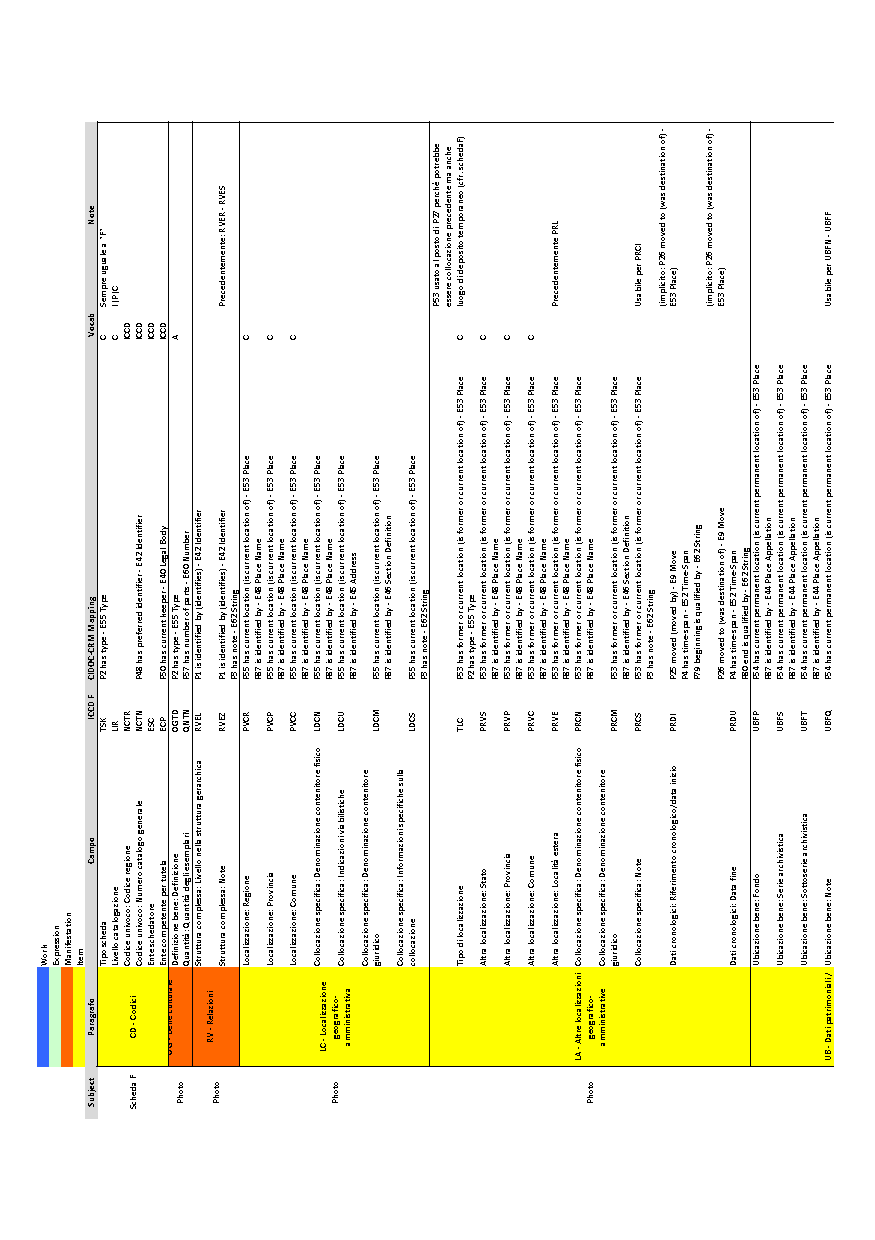
\includegraphics{images/Mapping-v3-1.pdf}
	\caption{Mappatura iniziale - 1}
	\label{fig:mapping-v3-1}
\end{figure}
\begin{figure}[ht!]
    \centering
    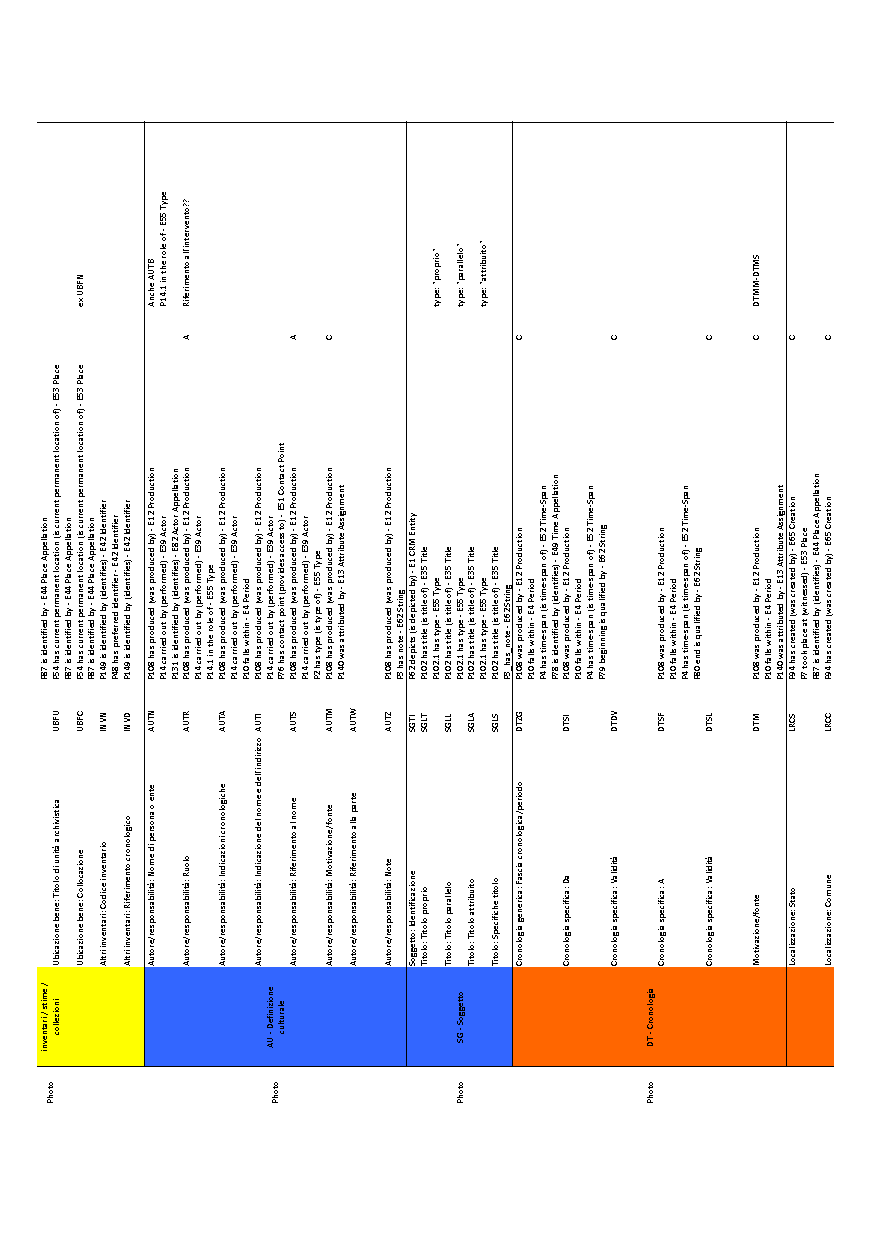
\includegraphics{images/Mapping-v3-2.pdf}
	\caption{Mappatura iniziale - 2}
	\label{fig:mapping-v3-2}
\end{figure}
\begin{figure}[ht!]
    \centering
    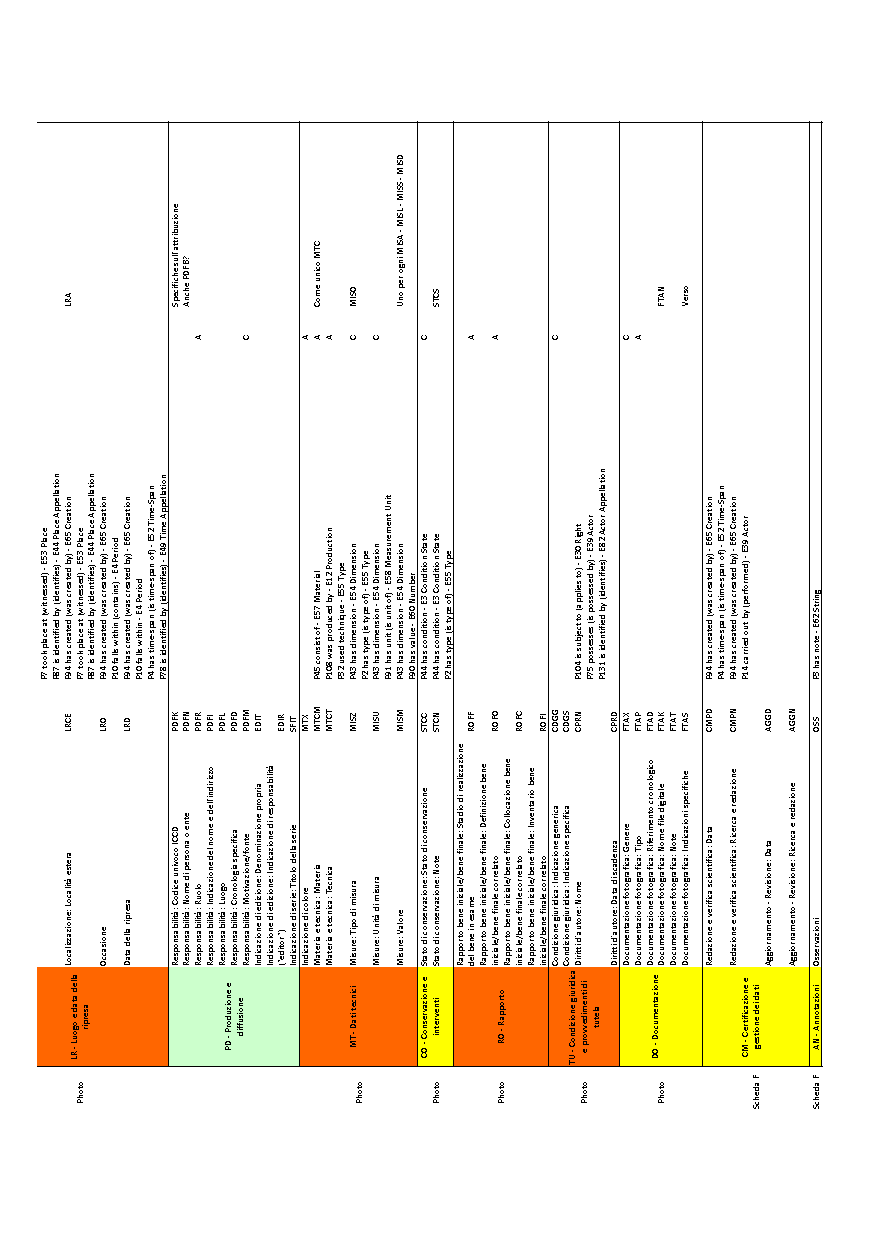
\includegraphics{images/Mapping-v3-3.pdf}
	\caption{Mappatura iniziale - 3}
	\label{fig:mapping-v3-3}
\end{figure}
\end{center}

